%% Преамбула TeX-файла

% 1. Стиль и язык
\documentclass[utf8x]{G7-32} % Стиль (по умолчанию будет 14pt)
\usepackage[T2A]{fontenc}
\usepackage[russian]{babel}
% Остальные стандартные настройки убраны в preamble.inc.tex.
\sloppy

% Настройки стиля ГОСТ 7-32
% Для начала определяем, хотим мы или нет, чтобы рисунки и таблицы нумеровались в пределах раздела, или нам нужна сквозная нумерация.
\EqInChapter % формулы будут нумероваться в пределах раздела
\TableInChapter % таблицы будут нумероваться в пределах раздела
\PicInChapter % рисунки будут нумероваться в пределах раздела

% Добавляем гипертекстовое оглавление в PDF
\usepackage[
bookmarks=true, colorlinks=true, unicode=true,
urlcolor=black,linkcolor=black, anchorcolor=black,
citecolor=black, menucolor=black, filecolor=black,
]{hyperref}

% Изменение начертания шрифта --- после чего выглядит таймсоподобно.
% apt-get install scalable-cyrfonts-tex

\IfFileExists{cyrtimes.sty}
    {
        \usepackage{cyrtimespatched}
    }
    {
        % А если Times нету, то будет CM...
    }

\usepackage{graphicx}   % Пакет для включения рисунков

% С такими оно полями оно работает по-умолчанию:
% \RequirePackage[left=20mm,right=10mm,top=20mm,bottom=20mm,headsep=0pt]{geometry}
% Если вас тошнит от поля в 10мм --- увеличивайте до 20-ти, ну и про переплёт не забывайте:
\geometry{right=20mm}
\geometry{left=30mm}


% Пакет Tikz
\usepackage{tikz}
\usetikzlibrary{arrows,positioning,shadows}

% Произвольная нумерация списков.
\usepackage{enumerate}

% ячейки в несколько строчек
\usepackage{multirow}

% itemize внутри tabular
\usepackage{paralist,array}


% Настройки листингов.
% 8 Листинги

\usepackage{listings}

% Значения по умолчанию
\lstset{
  basicstyle= \footnotesize,
  breakatwhitespace=true,% разрыв строк только на whitespacce
  breaklines=true,       % переносить длинные строки
%   captionpos=b,          % подписи снизу -- вроде не надо
  inputencoding=koi8-r,
  numbers=left,          % нумерация слева
  numberstyle=\footnotesize,
  showspaces=false,      % показывать пробелы подчеркиваниями -- идиотизм 70-х годов
  showstringspaces=false,
  showtabs=false,        % и табы тоже
  stepnumber=1,
  tabsize=4,              % кому нужны табы по 8 символов?
  frame=single
}

% Стиль для псевдокода: строчки обычно короткие, поэтому размер шрифта побольше
\lstdefinestyle{pseudocode}{
  basicstyle=\small,
  keywordstyle=\color{black}\bfseries\underbar,
  language=Pseudocode,
  numberstyle=\footnotesize,
  commentstyle=\footnotesize\it
}

% Стиль для обычного кода: маленький шрифт
\lstdefinestyle{realcode}{
  basicstyle=\scriptsize,
  numberstyle=\footnotesize
}

% Стиль для коротких кусков обычного кода: средний шрифт
\lstdefinestyle{simplecode}{
  basicstyle=\footnotesize,
  numberstyle=\footnotesize
}

% Стиль для BNF
\lstdefinestyle{grammar}{
  basicstyle=\footnotesize,
  numberstyle=\footnotesize,
  stringstyle=\bfseries\ttfamily,
  language=BNF
}

% Определим свой язык для написания псевдокодов на основе Python
\lstdefinelanguage[]{Pseudocode}[]{Python}{
  morekeywords={each,empty,wait,do},% ключевые слова добавлять сюда
  morecomment=[s]{\{}{\}},% комменты {а-ля Pascal} смотрятся нагляднее
  literate=% а сюда добавлять операторы, которые хотите отображать как мат. символы
    {->}{\ensuremath{$\rightarrow$}~}2%
    {<-}{\ensuremath{$\leftarrow$}~}2%
    {:=}{\ensuremath{$\leftarrow$}~}2%
    {<--}{\ensuremath{$\Longleftarrow$}~}2%
}[keywords,comments]

% Свой язык для задания грамматик в BNF
\lstdefinelanguage[]{BNF}[]{}{
  morekeywords={},
  morecomment=[s]{@}{@},
  morestring=[b]",%
  literate=%
    {->}{\ensuremath{$\rightarrow$}~}2%
    {*}{\ensuremath{$^*$}~}2%
    {+}{\ensuremath{$^+$}~}2%
    {|}{\ensuremath{$|$}~}2%
}[keywords,comments,strings]

% Подписи к листингам на русском языке.
\renewcommand\lstlistingname{\cyr\CYRL\cyri\cyrs\cyrt\cyri\cyrn\cyrg}
\renewcommand\lstlistlistingname{\cyr\CYRL\cyri\cyrs\cyrt\cyri\cyrn\cyrg\cyri}


% Полезные макросы листингов.
% Любимые команды

\usepackage{hyperref}


\newtheorem{theorem}{Теорема}
\newtheorem{definition}{Определение}

\newcommand{\Code}[1]{\textbf{#1}}


\newcommand{\myImage}[3]{
\begin{figure}[!ht]
    \centering
    \includegraphics[width=0.85\textwidth]{figures/#2}
    \caption{#1}
    \label{#3}
\end{figure}
}


\begin{document}

\pagestyle{empty}
\begin{center}
    Министерство образования и науки Российской Федерации\\
    ФГАОУ ВПО  «УрФУ имени первого Президента России Б. Н. Ельцина»\\
    Институт радиоэлектроники и информационных технологий - РтФ\\
    Департамент информационных технологий и автоматики
    \par
    \vspace{4.5cm}
    \Large{
      Иммитационное моделирование в  системе Bizagi Proces Modeler

      \par
      \vspace{0.5cm}

      ОТЧЕТ\\
      по лабораторной работе
    }

    \vspace{4cm}
    {
      Преподаватель: \hfill Клебанов Борис Исаевич
    }
    \par
    {
      Студент: \hfill Сухоплюев Илья Владимирович
    }
    \par
    {
      Группа: \hfill РИ-440001
    }

    \par
    \vspace{3.5cm}
    Екатеринбург\\
    2017
\end{center}


\frontmatter % выключает нумерацию ВСЕГО; здесь начинаются ненумерованные главы: реферат, введение, глоссарий, сокращения и прочее.

% Команды \breakingbeforechapters и \nonbreakingbeforechapters
% управляют разрывом страницы перед главами.
% По-умолчанию страница разрывается.

% \nobreakingbeforechapters
% \breakingbeforechapters

\pagestyle{plain}

\tableofcontents

\Introduction

Целью работы является создание всякой всячины. Для достижения поставленной цели необходимо решить следующие задачи:

\begin{itemize}
\item проанализировать существующую всячину;
\item спроектировать свою, новую всячину;
\item изготовить всякую всячину;
\item проверить её работоспособность.
\end{itemize}

Вот так-то. А этот абзац вставлен для визуальной оценки отступа от перечня до следующего абзаца.

\mainmatter % это включает нумерацию глав и секций в документе ниже

\chapter{Описание и валидация бизнес-процесса}

\section{Описание бизнес процесса}

Для начала бегло рассмотрим процесс оказания услуги <<Совет
да любовь>>. Данная услуга оказывается гражданам, прожившим
в браке на территории Свердловской области 50 лет, которые
в силу этого могут быть представлены к награде <<Совет да любовь>>.
Наша услуга подготавливает наградной лист и предложения об
этом достяжении и передает их в правительство.

Начинается все с подачи документов заявителем в многофункциональный
центр, там документы регистрируются и передаются в министерство
Социальной политики Сверловской области (далее, министерство).
Там, если заявителем не были предоставлены сведения о судимости,
отправляется запрос в Информационный центр (ИЦ).
После получения этих сведений, проверяется соблюдения прав
и свобод детей у заявителей. Для этого требуется согласование
с терроториальной комиссией по делам несовершенолетних
и защите их прав (ТКДНиЗП). И согласовав данный этап,
в министерстве оформляется наградной лист и предложения
о награждении, и они передаются в Правительство Свердловской
области.

\clearpage
\section{Создание диаграммы процесса}

Описав кратко моделируемую услугу, перейдем к описанию
этого бизнес-процесса в виде нотации BPMN (Рисунок \ref{description}).

Все элементы процесса размещаются в пуле процесса, который
делится на дорожки, где каждая дорожка представляет исполнителя.
В нашем случе это: заявитель, МФЦ, министерство, ИЦ и ТКДНиЗП.

Бизнес-процесс начинается со стартового события,
зеленого круга (подача заявления), и заканчивается
завершающимся событием, крсным кругом (передача предложений и
наградного листа в Правительство). Между этими событиями
происходит передача управления на выполнение промежуточных
задач, синих прямоугольников.

В добавок к этому, в нашей схеме содержится шлюз, на котором
управление передается в зависимости от того, были
ли в подоваемых документах сведения о судмости заявителей или нет.

Если этих требований не было, то происходит передача сообщений
в информационный центр и обратно. Внутри него данные сведения
могут быть получены разными способами, поэтому данная задача
описана, как комплексная.

\begin{sidewaysfigure}
    \centering
    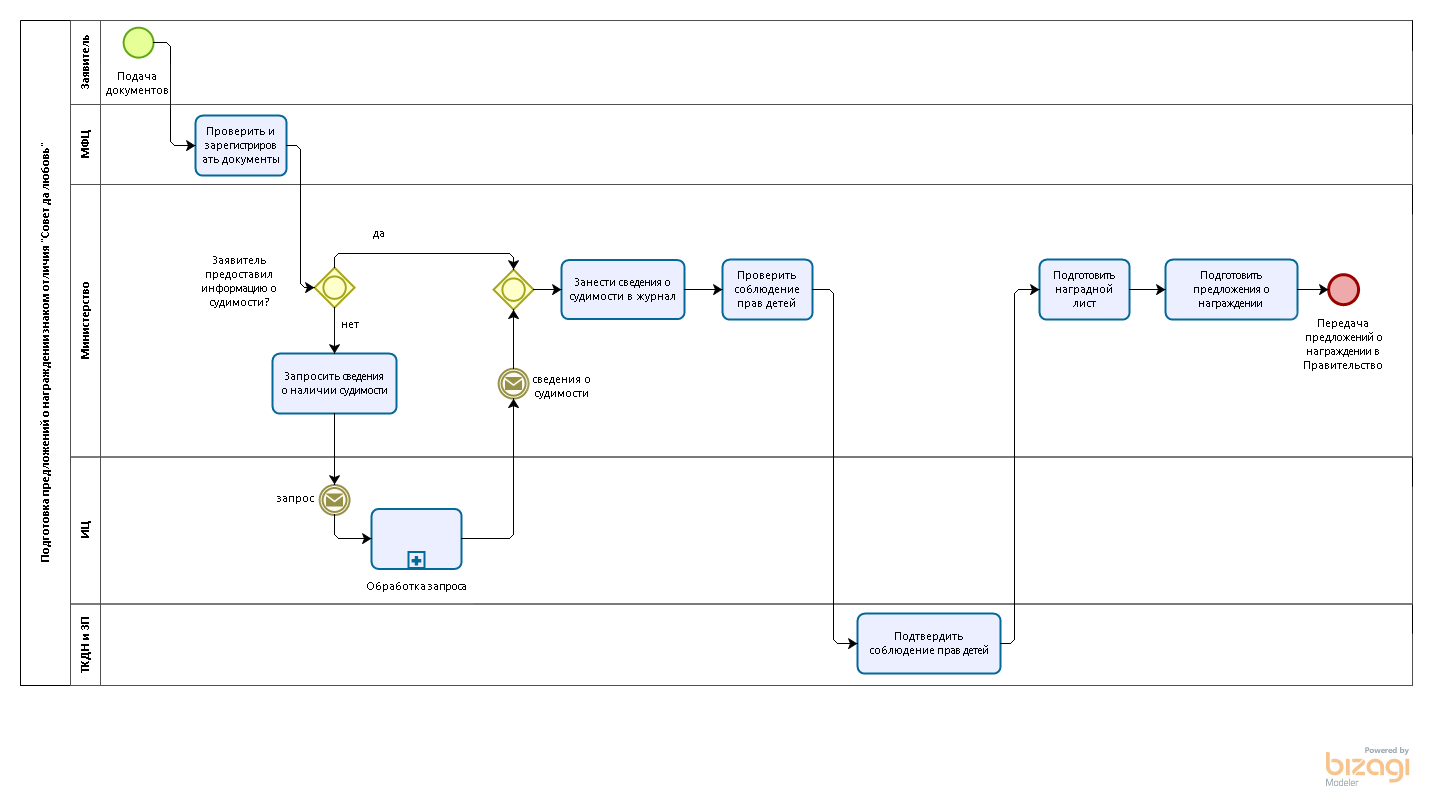
\includegraphics[width=\textwidth]{figures/model-description}
    \caption{Улуга <<Совет да любовь>> в нотации BPMN}
    \label{description}
\end{sidewaysfigure}

\clearpage
\section{Запуск моделирования}

Теперь, чтобы проверить корректность описания этапов нашего
процесса в нотации BPMN, мы можем запустить моделирование на
первом этапе (\textit{Process Validation}).

Для этого, нам нужно создать поток входных заявок в у
начального события, нажав на шестеренку рядом (Рис. \ref{run:flow}).
А также указать, в каком отношении соотносятся события,
происходящие на шлюзе (Рис. \ref{run:gate}): в нашем случае
мы считаем, что 90 \% заявителей не приносят сведения о судимости
при подачи заявления.
\myImage{Задание потока заявок на входе модели}{run_control}{run:flow}
\myImage{Задание вероятносного распределения на шлюзе}{run_if}{run:gate}
\clearpage

\myImage{Вывод отчета о проведенном моделировании}{run_report}{run:report}

Этого достаточно, чтобы запустить иммитацию процесса: перходим
в вид \textit{Simulation View} и нажимаем \textit{Run}.
В результате нам показывается отчет выполнения имитации (Рис. \ref{run:report}),
на котором мы видим количество пройденых заявок на каждом этапе.
Несмотря на большое количество согласований и проверок в нашем
процессе (проверка сведений о судимости, проверка соблюдения
прав детей), в регламенте услуги сказано, что нет никаких причин
в отказе оказания услуги, то есть она является этапом на котором
формируется вся необходимая информация. Поэтому количество
заявок на начальном событии должно быть равно количеству
заявок на конечном этапе, что выделено на рисунке.
Таким образом модель процесса составлена корректно.

\chapter{Временной анализ}

Проверив составленную модель на валидность, перейдем
к следующему этапу анализа - временому. В этом анализе
мы опишем, сколько времени выполняется каждая подзадача
и оценим, как эффективно выполняется процесс с этими
ограничениями.

В таблице \ref{table:time} представлены временные затарты
на простые задачи, присутствующие в нашей схеме. Задать их
в Bizagi Modeler очень просто: достаточно нажать на значек
часов справа от задачи, после чего ввести требуемое время
(Рисунок \ref{time_set}).

\begin{table}
    \begin{tabular}{|l|c|}
        \hline
        Проверить и зарегистрировать документы & 15min \\ \hline
        Запросить сведения о наличии судимости & 30min \\ \hline
        Занести сведения о судимости в журнал & 10min \\ \hline
        Проверить соблюдение прав детей & 30min \\ \hline
        Подтвердить соблюдение прав детей & 6hours \\ \hline
        Подготовить наградной лист & 2hours \\ \hline
        Подготовить предложения о награждении & 2hours \\ \hline
    \end{tabular}
    \caption{Время выполнения подзадач в процессе}
    \label{table:time}
\end{table}

\myImage{Задание времени выполнения элементарной задачи
}{time_set}{time_set}
\clearpage

\myImage{Задание времени выполнения обработки запроса в ИЦ
с помощью нормального распределения}{time_randn}{time_randn}

В предыдущей таблице мы не рассмотрели один этап -
обработку запроса в ИЦ на наличие судимости о заявителя.
Так как это сложный процесс, и нам неизвестна внутренняя
структура обработки запроса, смоделируем его время выполнения
как нормальное распределение (Рисунок \ref{time_randn}).
Будем считать, что в среднем обработка запроса будет
4-ре дня (5760 минут) со стандартным отклонением в 1000 минут
(~0.7дня).

Запустив заполненую модель в режиме временого анализа,
мы получем новый, более детальный, отчет (Рисунок
\ref{time_report}). Тут больше всего нас интерисуют колонки
времени выполнения каждого этапа задачи (минимальное,
максимально и среднее на каждую задачу).

Отсортировав по среднему времени выполнения задачи,
можно отчетливо видить узкое горлышко нашего процесса -
среднее время выполнения почти полностью требуется на обработку
запроса в информационном центре. При этом, если повезет,
данная процедура может пройти за 10 часов, при условии, что
заявитель предоставил эти сведения о судимости
при регистрации документов.

\myImage{Отчет симуляции для анализа времени, затраченного
на бизнес-процесс}{time_report}{time_report}

\chapter{Анализ используемых ресурсов}

\chapter{Календарный анализ}

\chapter{Анализ <<Что-Если>>}

Теперь попробуем промоделировать очевидное решение проблемы,
наблюдаемой нами в ходе всех этапов анализа: долгое время
обработки и подготовки сведений о судимости в информационном центре.

Для этого воспользуемся еще одной замечательной возможностью
Bizagi Modeler: \textit{What-If-Analysis} или Анализ Что-Если.
В процессе его проведения, мы создадем копию моделируемого
процесса (Рис. \ref{what-if}), после чего вносим в копию
модели правки, которые желаем провести в бизнес-процессе.
Далее программа сама может быстро провести оба моделирвоания,
и предоставить сравнительный отчет работы этих двух систем.

В нашем случае, представим, что информационный центр
модернизировали и сделали обработку требуемого запроса
автоматической с помощью сервиса, который способен выполнить
его в течении 5 минут, при этом возможна обработка до 100
одновременных запросов.

Запустив анализ мы получаем отчет (Рисунки
\ref{what-if-resources-report},
\ref{what-if-common-report},
\ref{what-if-inc-report} и
\ref{what-if-inc-report-2}). Как можем заметить, нагрузка на
ИЦ упала до 0.04\%, что вполне ожидаемо. Однако мы не
получили значительного повышения производительности в бизнес
процессе: да, максимальное время выполнение уменьшилось и
составляет 61-62 дня, что приемлемо для нашего регламента,
однако же среднее время выполнения увеличилось на целых два
дня.

В чем же такая значительная проблема? Просмотрев другие задачи,
можно увидеть, что из-за быстрой обработки запросов
информационным центром, большой поток заявок нагрузил других
исполнителей процесса, что вызвало задержки ожидания работников,
что в конечном счете повлияло на среднее время выполнение почти
что всех задач не в лучшую сторону. И таким образом,
выигрышь 30 дней задержки при обработке информационным центром
оказался не таким значительным, как ожидалось.

\myImage{Создание копии модели процесса}{what-if}{what-if}
\myImage{Сравнительный отчет ресурсов: нагрузка на ИЦ заментно снизилась
}{what-if-resources-report}{what-if-resources-report}
\myImage{Максимальное время выполнения уменьшилось до
допустимых пределов, чего не скажешь о среднем времени
выполнения запроса}{what-if-common-report}{what-if-common-report}
\myImage{Как видно среденее время выполнения других задач
существенно выросло}{what-if-inc-report}{what-if-inc-report}
\myImage{Виден выигрыш в 30 дней на обработке запроса в ИЦ,
как и увеличение среднего времени выполнения оставшихся
задач}{what-if-inc-report-2}{what-if-inc-report-2}




\backmatter %% Здесь заканчивается нумерованная часть документа и начинаются ссылки и
            %% заключение

\Conclusion % заключение к отчёту

В ходе проделанной лабораторной работы, был изучен и
смоделирован бизнес-процесс оказания государственной
услуги <<Совет да любовь>>. В ходе этого моделирования,
удалось на практике ознакомится с методами анализа,
предоставляемыми Bizagi Process Modeler: описание
процесса в натации стандарта BPMN 2.0, временной анализ,
анализ затрат ресурсов, а также календарный анализ.

Во время проведения моделирования, было найдено одно
узкое место в моделируемом процессе -- обработка запроса
через ИЦ. После этого был проведен эксперимент в виде
сравнительного анализа "Что-Если", в котором мы
попытались проверить гипотезу, что процесс значительно
улучшится, если мы модернезируем ИЦ.

В результате этого анализа программа Bizagi Modeler
предоставила нам сравнительные таблицы, по которым мы пришли
к неоднозначным результатам: с одной стороны максимальное
время оказания услуги уменьшилось и стало допустимым с другой
среднее время выполнения увеличилось, за счет задержек
возникших на других этапах решения задачи.

Таким образом, требуется провести более комплексные экспеименты,
чтобы значительно повлиять на работу данного процесса.




%%% Local Variables:
%%% mode: latex
%%% TeX-master: "rpz"
%%% End:


% % Список литературы при помощи BibTeX
% Юзать так:
%
% pdflatex rpz
% bibtex rpz
% pdflatex rpz

\bibliographystyle{gost780u}
\bibliography{rpz}

%%% Local Variables: 
%%% mode: latex
%%% TeX-master: "rpz"
%%% End: 


\appendix   % Тут идут приложения

\end{document}

%%% Local Variables:
%%% mode: latex
%%% TeX-master: t
%%% End:
